\documentclass{standalone}
\usepackage{tikz}
\usetikzlibrary{patterns, positioning}

\begin{document}
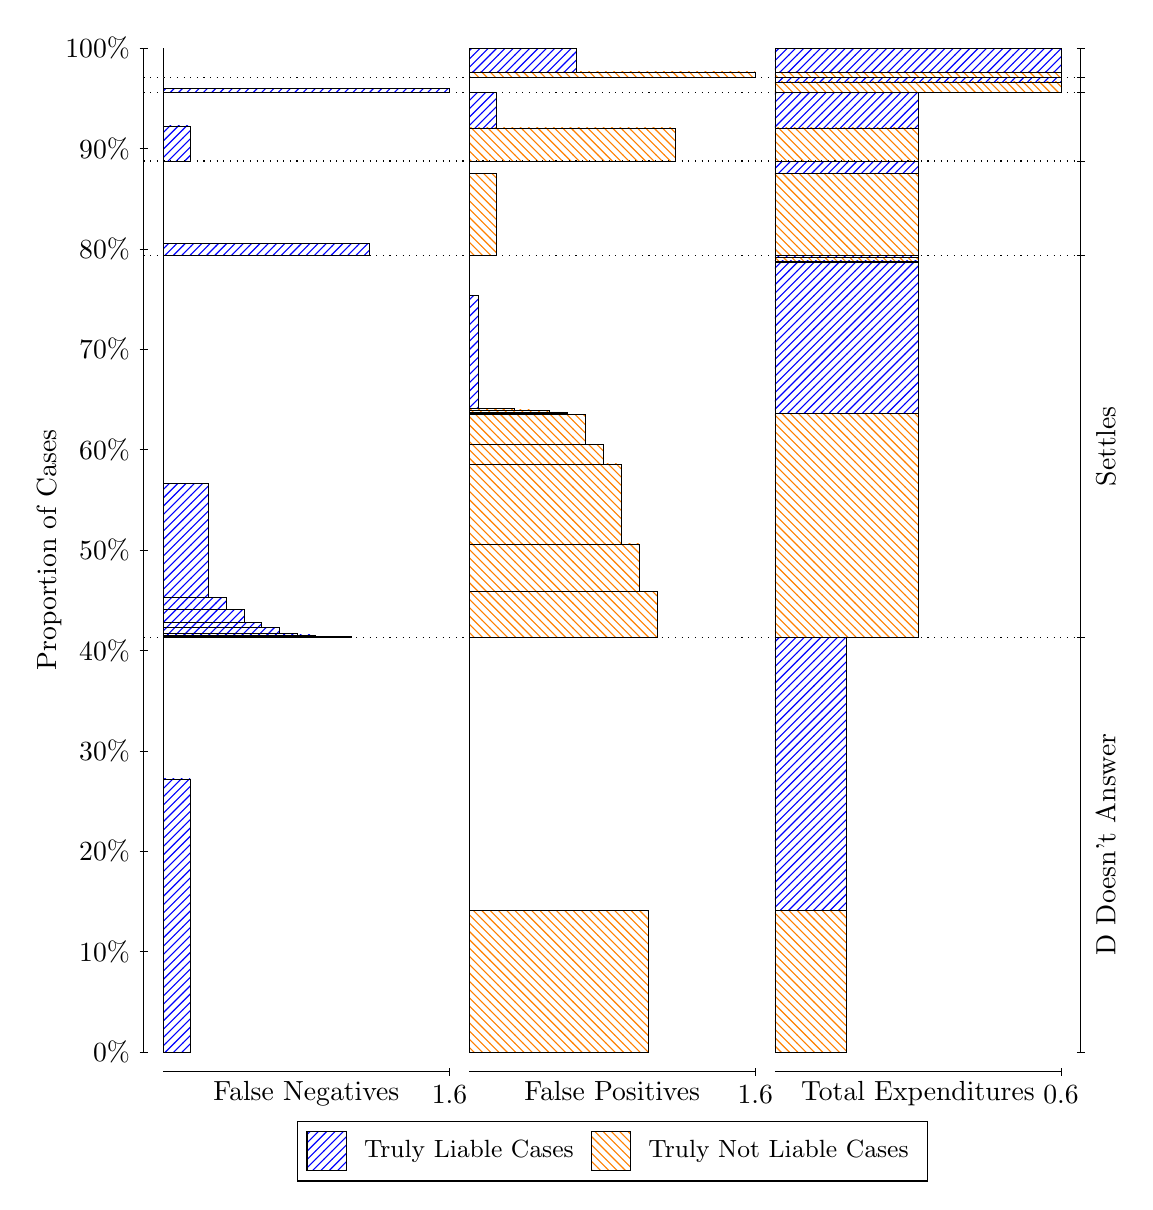
\begin{tikzpicture}
\draw[black, very thin] (1.5,1.75) -- (1.5,14.5);
\node[rotate=90, anchor=center] at (0.3, 8.125) {Proportion of Cases};
\draw[black, very thin] (1.45,1.75) -- (1.55,1.75);
\node[anchor=east] at (1.45, 1.75) {0\%};
\draw[black, very thin] (1.45,3.025) -- (1.55,3.025);
\node[anchor=east] at (1.45, 3.025) {10\%};
\draw[black, very thin] (1.45,4.3) -- (1.55,4.3);
\node[anchor=east] at (1.45, 4.3) {20\%};
\draw[black, very thin] (1.45,5.575) -- (1.55,5.575);
\node[anchor=east] at (1.45, 5.575) {30\%};
\draw[black, very thin] (1.45,6.85) -- (1.55,6.85);
\node[anchor=east] at (1.45, 6.85) {40\%};
\draw[black, very thin] (1.45,8.125) -- (1.55,8.125);
\node[anchor=east] at (1.45, 8.125) {50\%};
\draw[black, very thin] (1.45,9.4) -- (1.55,9.4);
\node[anchor=east] at (1.45, 9.4) {60\%};
\draw[black, very thin] (1.45,10.675) -- (1.55,10.675);
\node[anchor=east] at (1.45, 10.675) {70\%};
\draw[black, very thin] (1.45,11.95) -- (1.55,11.95);
\node[anchor=east] at (1.45, 11.95) {80\%};
\draw[black, very thin] (1.45,13.225) -- (1.55,13.225);
\node[anchor=east] at (1.45, 13.225) {90\%};
\draw[black, very thin] (1.45,14.5) -- (1.55,14.5);
\node[anchor=east] at (1.45, 14.5) {100\%};

\draw[black, very thin] (13.4,1.75) -- (13.4,14.5);
\draw[black, very thin] (13.35,1.75) -- (13.45,1.75);
\node[anchor=west] at (13.35, 1.75) {};
\draw[black, very thin] (13.35,7.0182) -- (13.45,7.0182);
\node[anchor=west] at (13.35, 7.0182) {};
\draw[black, very thin] (13.35,11.867) -- (13.45,11.867);
\node[anchor=west] at (13.35, 11.867) {};
\draw[black, very thin] (13.35,13.065) -- (13.45,13.065);
\node[anchor=west] at (13.35, 13.065) {};
\draw[black, very thin] (13.35,13.932) -- (13.45,13.932);
\node[anchor=west] at (13.35, 13.932) {};
\draw[black, very thin] (13.35,14.125) -- (13.45,14.125);
\node[anchor=west] at (13.35, 14.125) {};
\draw[black, very thin] (13.35,14.5) -- (13.45,14.5);
\node[anchor=west] at (13.35, 14.5) {};

\draw[black, very thin, pattern color=blue, pattern=north east lines] (1.75,1.75) rectangle (2.0906,5.217);
\draw[black, very thin, pattern color=orange, pattern=north west lines] (1.75,5.217) rectangle (1.75,7.0182);
\draw[black, very thin, pattern color=blue, pattern=north east lines] (1.75,7.0182) rectangle (4.1344,7.0263);
\draw[black, very thin, pattern color=blue, pattern=north east lines] (1.75,7.0263) rectangle (3.9073,7.0324);
\draw[black, very thin, pattern color=blue, pattern=north east lines] (1.75,7.0324) rectangle (3.6802,7.0468);
\draw[black, very thin, pattern color=blue, pattern=north east lines] (1.75,7.0468) rectangle (3.4531,7.0612);
\draw[black, very thin, pattern color=blue, pattern=north east lines] (1.75,7.0612) rectangle (3.226,7.1438);
\draw[black, very thin, pattern color=blue, pattern=north east lines] (1.75,7.1438) rectangle (2.999,7.2085);
\draw[black, very thin, pattern color=blue, pattern=north east lines] (1.75,7.2085) rectangle (2.7719,7.3715);
\draw[black, very thin, pattern color=blue, pattern=north east lines] (1.75,7.3715) rectangle (2.5448,7.5244);
\draw[black, very thin, pattern color=blue, pattern=north east lines] (1.75,7.5244) rectangle (2.3177,8.9661);
\draw[black, very thin, pattern color=orange, pattern=north west lines] (1.75,8.9661) rectangle (1.75,11.867);
\draw[black, very thin, pattern color=blue, pattern=north east lines] (1.75,11.867) rectangle (4.3615,12.022);
\draw[black, very thin, pattern color=orange, pattern=north west lines] (1.75,12.022) rectangle (1.75,13.065);
\draw[black, very thin, pattern color=blue, pattern=north east lines] (1.75,13.065) rectangle (2.0906,13.511);
\draw[black, very thin, pattern color=orange, pattern=north west lines] (1.75,13.511) rectangle (1.75,13.932);
\draw[black, very thin, pattern color=blue, pattern=north east lines] (1.75,13.932) rectangle (5.3833,13.987);
\draw[black, very thin, pattern color=orange, pattern=north west lines] (1.75,13.987) rectangle (1.75,14.125);
\draw[black, very thin, pattern color=orange, pattern=north west lines] (1.75,14.125) rectangle (1.75,14.196);
\draw[black, very thin, pattern color=blue, pattern=north east lines] (1.75,14.196) rectangle (1.75,14.5);
\draw[black, very thin, pattern color=orange, pattern=north west lines] (5.6333,1.75) rectangle (7.9042,3.5511);
\draw[black, very thin, pattern color=blue, pattern=north east lines] (5.6333,3.5511) rectangle (5.6333,7.0182);
\draw[black, very thin, pattern color=orange, pattern=north west lines] (5.6333,7.0182) rectangle (8.0177,7.5968);
\draw[black, very thin, pattern color=orange, pattern=north west lines] (5.6333,7.5968) rectangle (7.7906,8.2028);
\draw[black, very thin, pattern color=orange, pattern=north west lines] (5.6333,8.2028) rectangle (7.5635,9.22);
\draw[black, very thin, pattern color=orange, pattern=north west lines] (5.6333,9.22) rectangle (7.3365,9.4644);
\draw[black, very thin, pattern color=orange, pattern=north west lines] (5.6333,9.4644) rectangle (7.1094,9.8511);
\draw[black, very thin, pattern color=orange, pattern=north west lines] (5.6333,9.8511) rectangle (6.8823,9.8641);
\draw[black, very thin, pattern color=orange, pattern=north west lines] (5.6333,9.8641) rectangle (6.8823,9.8732);
\draw[black, very thin, pattern color=orange, pattern=north west lines] (5.6333,9.8732) rectangle (6.6552,9.896);
\draw[black, very thin, pattern color=orange, pattern=north west lines] (5.6333,9.896) rectangle (6.4281,9.9058);
\draw[black, very thin, pattern color=orange, pattern=north west lines] (5.6333,9.9058) rectangle (6.201,9.9188);
\draw[black, very thin, pattern color=blue, pattern=north east lines] (5.6333,9.9188) rectangle (5.7469,11.361);
\draw[black, very thin, pattern color=blue, pattern=north east lines] (5.6333,11.361) rectangle (5.6333,11.867);
\draw[black, very thin, pattern color=orange, pattern=north west lines] (5.6333,11.867) rectangle (5.974,12.91);
\draw[black, very thin, pattern color=blue, pattern=north east lines] (5.6333,12.91) rectangle (5.6333,13.065);
\draw[black, very thin, pattern color=orange, pattern=north west lines] (5.6333,13.065) rectangle (8.2448,13.485);
\draw[black, very thin, pattern color=blue, pattern=north east lines] (5.6333,13.485) rectangle (5.974,13.932);
\draw[black, very thin, pattern color=orange, pattern=north west lines] (5.6333,13.932) rectangle (5.6333,14.069);
\draw[black, very thin, pattern color=blue, pattern=north east lines] (5.6333,14.069) rectangle (5.6333,14.125);
\draw[black, very thin, pattern color=orange, pattern=north west lines] (5.6333,14.125) rectangle (9.2667,14.196);
\draw[black, very thin, pattern color=blue, pattern=north east lines] (5.6333,14.196) rectangle (6.9958,14.5);
\draw[black, very thin, pattern color=orange, pattern=north west lines] (9.5167,1.75) rectangle (10.425,3.5511);
\draw[black, very thin, pattern color=blue, pattern=north east lines] (9.5167,3.5511) rectangle (10.425,7.0182);
\draw[black, very thin, pattern color=orange, pattern=north west lines] (9.5167,7.0182) rectangle (11.333,9.8641);
\draw[black, very thin, pattern color=blue, pattern=north east lines] (9.5167,9.8641) rectangle (11.333,11.777);
\draw[black, very thin, pattern color=orange, pattern=north west lines] (9.5167,11.777) rectangle (11.333,11.79);
\draw[black, very thin, pattern color=blue, pattern=north east lines] (9.5167,11.79) rectangle (11.333,11.798);
\draw[black, very thin, pattern color=orange, pattern=north west lines] (9.5167,11.798) rectangle (11.333,11.84);
\draw[black, very thin, pattern color=blue, pattern=north east lines] (9.5167,11.84) rectangle (11.333,11.867);
\draw[black, very thin, pattern color=orange, pattern=north west lines] (9.5167,11.867) rectangle (11.333,12.91);
\draw[black, very thin, pattern color=blue, pattern=north east lines] (9.5167,12.91) rectangle (11.333,13.065);
\draw[black, very thin, pattern color=orange, pattern=north west lines] (9.5167,13.065) rectangle (11.333,13.485);
\draw[black, very thin, pattern color=blue, pattern=north east lines] (9.5167,13.485) rectangle (11.333,13.932);
\draw[black, very thin, pattern color=orange, pattern=north west lines] (9.5167,13.932) rectangle (13.15,14.069);
\draw[black, very thin, pattern color=blue, pattern=north east lines] (9.5167,14.069) rectangle (13.15,14.125);
\draw[black, very thin, pattern color=orange, pattern=north west lines] (9.5167,14.125) rectangle (13.15,14.196);
\draw[black, very thin, pattern color=blue, pattern=north east lines] (9.5167,14.196) rectangle (13.15,14.5);
\draw[black, dotted] (1.5,7.0182) -- (13.4,7.0182);
\draw[black, dotted] (1.5,11.867) -- (13.4,11.867);
\draw[black, dotted] (1.5,13.065) -- (13.4,13.065);
\draw[black, dotted] (1.5,13.932) -- (13.4,13.932);
\draw[black, dotted] (1.5,14.125) -- (13.4,14.125);
\draw[black, very thin] (1.75,1.5) -- (5.3833,1.5);
\node[anchor=north] at (3.5667, 1.5) {False Negatives};
\draw[black, very thin] (5.3833,1.45) -- (5.3833,1.55);
\node[anchor=north] at (5.3833, 1.45) {1.6};

\draw[black, very thin] (5.6333,1.5) -- (9.2667,1.5);
\node[anchor=north] at (7.45, 1.5) {False Positives};
\draw[black, very thin] (9.2667,1.45) -- (9.2667,1.55);
\node[anchor=north] at (9.2667, 1.45) {1.6};

\draw[black, very thin] (9.5167,1.5) -- (13.15,1.5);
\node[anchor=north] at (11.333, 1.5) {Total Expenditures};
\draw[black, very thin] (13.15,1.45) -- (13.15,1.55);
\node[anchor=north] at (13.15, 1.45) {0.6};

\node[black, centered, rotate=90] at (13.72, 4.3841) {D Doesn't Answer};
\node[black, centered, rotate=90] at (13.72, 9.4425) {Settles};





\draw (7.449999999999999,1.5) node[draw=none] (baseCoordinate) {};
\begin{scope}[align=center]
        \matrix[scale=0.5, draw=black, below=0.5cm of baseCoordinate, nodes={draw}, column sep=0.1cm]{
            \node[rectangle, draw, minimum width=0.5cm, minimum height=0.5cm, pattern=north east lines, pattern color=blue] {}; &
            \node[draw=none, font=\small] (B) {Truly Liable Cases}; &
            \node[rectangle, draw, minimum width=0.5cm, minimum height=0.5cm, pattern=north west lines, pattern color=orange] {}; &
            \node[draw=none, font=\small] (B) {Truly Not Liable Cases}; \\
            };
\end{scope}

\end{tikzpicture}
\end{document}